\documentclass[12pt,a4paper,utf8]{ctexart}
\usepackage{graphicx}

\usepackage{amsmath}

\usepackage{amssymb}

\usepackage{subfig}

\usepackage{cite}
\usepackage[ntheorem]{empheq}
\usepackage{enumitem}
\usepackage{fullpage}
\usepackage{cleveref}
\usepackage{cellspace}
\usepackage{listings}
\usepackage{color}
\usepackage[top=2cm, bottom=2cm, left=2cm, right=2cm]{geometry}  
\usepackage{algorithm}  
\usepackage{algorithmicx}  
\usepackage{algpseudocode}  
\renewcommand{\algorithmicrequire}{\textbf{Input:}}  % Use Input in the format of Algorithm  
\renewcommand{\algorithmicensure}{\textbf{Output:}} % Use Output in the format of Algorithm 
\definecolor{gray}{rgb}{0.5,0.5,0.5}
\definecolor{dkgreen}{rgb}{.068,.578,.068}
\definecolor{dkpurple}{rgb}{.320,.064,.680}

% set Matlab styles
\lstset{
   language=Matlab,
   keywords={break,case,catch,continue,else,elseif,end,for,function,
      global,if,otherwise,persistent,return,switch,try,while},
   basicstyle=\small\ttfamily,
   keywordstyle=\color{blue}\bfseries,
   commentstyle=\color{dkgreen},
   stringstyle=\color{dkpurple},
   backgroundcolor=\color{white},
   tabsize=4,
   showspaces=false,
   showstringspaces=false
}

\begin{document}
\CJKfamily{zhkai}	


\begin{center}
\textbf{作业一}\\
\textbf{姓名:晏瑞然~~~~~~~~~~~~~ 学号:PB19000196~~~~~~~~~~~~~~ 日期:5.27}\\
\end{center}

\begin{center}
\fbox{
\begin{minipage}{40em}
\vspace{5cm}
\hspace{20cm}
\end{minipage}}
\end{center}
\vspace{1cm}

\begin{enumerate}
\item[第一题] \textbf{本题考虑对于定义在[−1, 1]上的一个光滑函数$f(x)$的三次样条插值的使用。下面
所说的误差都是指绝对误差}  

(a)(10分)仿照课堂笔记或课本推导出关于额外给定边界点处(即−1和1)
三次样条插值多项式的一次导数值时其在各插值点上的二次导数值应该满足的
线性方程组。请给出推导过程。
\newline

解:

记$S(x)$在区间$[x_i,x_{i+1}]$上的表达式是$S_i(x)$,$S(x)$是三次多项式,即$ S''(x) $ 是线型函数。
用插值点$ {(x_i,S''(x_i)),(x_{i+1},S''(x_{i+1}))}   $ 作线性插值,记$ S''(x_i)=M_i,S''(x_{i+1})=M_{i+1}. $ 
$$ S''_i(x) = \frac{x-x_{i+1}}{x_i-x_{i+1}} M_i + \frac{x-x_i}{x_{i+1}-x_i} M_{i+1}  ,\   x_i \leq x \leq x_{i+1} $$ 
对$ S''(x) $ 积分两次,记$ h_i=x_{i+1}-x_i, $ 
$$ S(x)=S_i(x)=\frac{(x_{i+1}-x)^3}{6h_i} M_i +\frac{(x-x_i)^3}{6h_i} M_{i+1} + cx + d $$
上式可进一步化简为:
$$ S(x)= \frac{(x_{i+1}-x)^3}{6h_i} M_i +\frac{(x-x_i)^3}{6h_i} M_{i+1} + C(x_{i+1}-x) + D(x-x_{i+1}) $$
将$ S(x_i)=y_i,S(x_{i+1})=y_{i+1} $带入上式解出:
$$ C=\frac{y_i}{h_i} -\frac{h_iM_i}{6} ,D = \frac{y_{i+1}}{h_i}-\frac{h_iM_{i+1}}{6}   $$ 
   
   \begin{equation}
      \begin{split}
         S(x) & = \frac{(x_{i+1}-x)^3M_i+(x-x_i)^3M_{i+1}}{6h_i} + \frac{(x_{i+1}-x)y_i+(x-x_i)y_{i+1}}{h_i}\\
         & -\frac{h_i}{6}[(x_{i+1}-x)M_{i}+(x-x_i)M_{i+1}] , \ x\in [x_i,x_{i+1}]
         \end{split}
      \end{equation}
         
又由$ S'_i(x_i)=S'_{i-1}(x(i)) $ 得
$$ f[x_i,x_{i+1}]-\frac{h_i}{3} M_i-\frac{h_i}{6} M_{i+1} = f[x_{i-1},x_{i}]-\frac{h_{i-1}}{3} M_{i-1}-\frac{h_{i-1}}{6} M_{i} $$ 
最后得
\begin{align}
   \mu_i M_{i-1}+2M_i+\lambda_i M_{i+1} = d_i , \ i=1,2,...,n-1 
\end{align}
其中
$$ \lambda_i = \frac{h_i}{h_i+h_{i-1}} , \ \mu_i=1-\lambda_i $$
$$ d_i = \frac{6}{h_i+h_{i-1}} (\frac{y_{i+1}-y_i}{h_i} - \frac{y_i-y_{i-1}}{h_{i-1}}) =6f[x_{i-1},x_i,x_{i+1}] $$

解式(2)可以得到$ M_i, \ i=1,2,...,M_{n-1} $ 再加上两个端点条件,就可以得到所有都M,最后带入式(1)即可得到$ [x_i,x_{i+1}] $ 上的样条插值函数$ S(x) $ 。

下面带入题目边界条件:

当给定一次导数值$S'(x_0)=m_0,S'(x_n)=m_n$时,将$S'(x_0)=m_0,S'(x_n)=m_n$带入$ S'(x) $ 在$ [x_0,x_1],[x_{n-1},x_n] $ 的表达式,得到另外两个方程:
$$ 2M_0+M_1 = \frac{6}{h_0} (f[x_0,x_1]-m_0)=d_0 $$
$$ M_{n-1}+2M_n = \frac{6}{h_{n-1}} (m_n-f[x_{n-1},x_n])=d_n $$
得到$ n+1 $ 个方程,矩阵表示为
\begin{equation}
   \left[
   \begin{array}{cccccccccccc}
    2    & 1 \\
    \mu_1& 2      & \lambda_1 \\
      \  & \mu_2  & 2      & \lambda_2 \\
      \  &   \    & \ddots & \ddots & \ddots \\
      \  &   \    &   \    & \mu_{n-1} & 2   &\lambda_{n-1} \\
      \  &   \    &   \    &     \     & 1   &2
   \end{array}
   \right ]
   \left[
   \begin{array}{cccc}
    M_{0}\\
    M_{1}\\
    M_{2}\\
    \vdots \\
    M_{n-1}\\
    M_{n}
   \end{array}
   \right ]
   =
   \left[
   \begin{array}{cccc}
      d_{0}\\
      d_{1}\\
      d_{2}\\
      \vdots \\
      d_{n-1}\\
      d_{n}
   \end{array}
   \right ]
   \end{equation}

(b)(10分)令三次样条插值多项式在−1和1处的导数为0,用Matlab基于上
一问中的结果使用$ n=2^4 $ 个子区间插值一个定义在[−1, 1]上的函数$ f(x) =sin(4x^2) + sin^2(4x) $并使用semilogy图通过在2000个等距点上取真实值画出你
构造的三次样条插值的逐点误差。

程序思路:

先划分区间,再由(a)中公式,得到$ \lambda_i,\mu_i,d_i $ 的值,构成系数矩阵A。
通过求解线性方程得到$ M_i $ 。最后带入式(1)得到分段函数$ S(x) $ 即可得到插值函数。
最后画出题目要求图像即可。

程序说明:

由于MATLAB中数组的序号是从1开始的而不是从0开始,所以要将(a)中推导的所有下标加1。
程序中表示分段函数的方式是先对所有的x求S(x),然后与其是否属于所属区间的逻辑值一一相乘,最后求和,即可得到分段函数。
具体方法见程序代码及代码注释。

结果图片:

\begin{figure}[htbp]
   \centering
   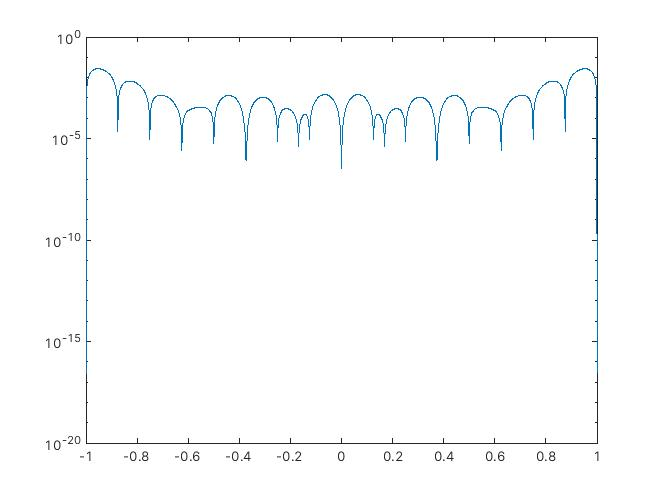
\includegraphics[width=15cm,height=8cm]{ex1b.jpg}
   \caption{第一题(b)}
\end{figure}

MATLAB程序如下:

主函数:
\begin{lstlisting}[frame=single]
n = 2^4; % 定义n
x = [-1:2/n:1]; % 得到区间端点x_i
% 得到h_i
h=[];
for i=1:n
    h=[h x(i+1)-x(i)];
end 
y=sin(4.*x.^2)+(sin(4.*x)).^2; % 得到y_i
% 初始化lambda,mu,d
lambda=ones(n,1);
mu=ones(n,1);
d=ones(n+1,1);
% 对除端点的lambda,mu,d赋值
for i=2:n
    lambda(i)=h(i)/(h(i)+h(i-1));
    mu(i)=1-lambda(i);
    d(i)=6/(h(i)+h(i-1))*((y(i+1)-y(i))/h(i) - (y(i)-y(i-1))/h(i-1));
end
% 对端点的lambda,mu,d赋值
d(1)=6/h(1)*((y(2)-y(1))/(x(2)-x(1))-0);
d(n+1)=6/h(n)*(0-(y(n+1)-y(n))/(x(n+1)-x(n)));
% 将所有的mu前移并将mu(n+1)赋值为1
mu(1)=[];
mu = [mu;1];
% 得到求解M的系数矩阵A
A=diag(mu,-1)+2.*eye(n+1)+diag(lambda,1);
M=A\d %得到M
x2=[-1:2/1999:1];% 分割2000个插值点
S=zeros(1,size(x2,1));% 初始化S
% 通过式(1)得到分段函数S
for i=1:n
    S=S+ ...
    (((x(i+1)-x2).^3*M(i)+(x2-x(i)).^3*M(i+1))/6/h(i) ...
    +((x(i+1)-x2)*y(i)+(x2-x(i))*y(i+1))/h(i) ...
    -(h(i)/6)*((x(i+1)-x2)*M(i)+(x2-x(i))*M(i+1)) ...
    ).*(x2>x(i)&x2<=x(i+1));% 分段函数即所有函数值.*其区间最后求和
end
% 单独得到S(1)
S(1)=((x(1+1)-x2(1)).^3*M(1)+(x2(1)-x(1)).^3*M(1+1))/6/h(1) ...
        +((x(1+1)-x2(1))*y(1)+(x2(1)-x(1))*y(1+1))/h(1) ...
        -(h(1)/6)*((x(1+1)-x2(1))*M(1)+(x2(1)-x(1))*M(1+1));
y2=sin(4.*x2.^2)+(sin(4.*x2)).^2;% 真实值
% 画图
figure
semilogy(x2,abs(y2-S))
   
\end{lstlisting}

(c):

求解方法与(b)一样,只是最后所求结果不同。
仍然是先求出插值的y然后与真实值相减。
最后求出最大误差值画出loglog图像。

\newpage
结果图片:
\begin{figure}[htbp]
   \centering
   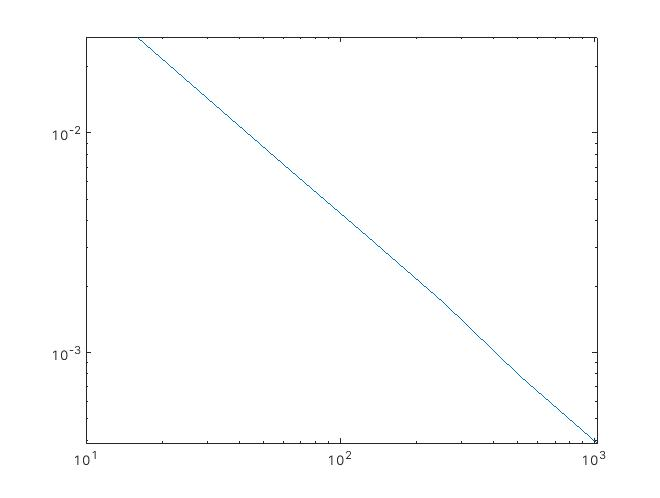
\includegraphics[width=15cm,height=8cm]{ex1c.jpg}
   \caption{第一题(c)}
\end{figure}



MATLAB程序如下:
\begin{lstlisting}[frame=single]
   err_max=zeros(1,7);% 初始化误差
   n2=[];% n2储存n值
   for exp=4:10
       n = 2^exp;% 定义n
       x = [-1:2/n:1];% 得到区间端点x_i
       % 得到h_i
       h=[];
       for i=1:n
           h=[h x(i+1)-x(i)];
       end 
       y=sin(4.*x.^2)+(sin(4.*x)).^2; % 得到y_i
       % 初始化lambda,mu,d
       lambda=ones(n,1);
       mu=ones(n,1);
       d=ones(n+1,1);
       % 对除端点的lambda,mu,d赋值
       for i=2:n
           lambda(i)=h(i)/(h(i)+h(i-1));
           mu(i)=1-lambda(i);
           d(i)=6/(h(i)+h(i-1))*((y(i+1)-y(i))/h(i) ... 
           - (y(i)-y(i-1))/h(i-1));
       end
       % 对端点的lambda,mu,d赋值
       d(1)=6/h(1)*((y(2)-y(1))/(x(2)-x(1))-0);
       d(n+1)=6/h(n)*(0-(y(n+1)-y(n))/(x(n+1)-x(n)));
       % 将所有的mu前移并将mu(n+1)赋值为1
       mu(1)=[];
       mu = [mu;1];
       % 得到求解M的系数矩阵A
       A=diag(mu,-1)+2.*eye(n+1)+diag(lambda,1);
       M=A\d;%得到M
       x2=[-1:2/1999:1];% 分割2000个插值点
       S=zeros(1,size(x2,1));% 初始化S
       % 通过式(1)得到分段函数S
       for i=1:n
           S=S+ ...
               (((x(i+1)-x2).^3*M(i)+(x2-x(i)).^3*M(i+1))/6/h(i) ...
               +((x(i+1)-x2)*y(i)+(x2-x(i))*y(i+1))/h(i) ...
               -(h(i)/6)*((x(i+1)-x2)*M(i)+(x2-x(i))*M(i+1)) ...
               ).*(x2>x(i)&x2<=x(i+1));
       end
       % 单独得到S(1)
       S(1)= ... 
      ((x(1+1)-x2(1)).^3*M(1)+(x2(1)-x(1)).^3*M(1+1))/6/h(1) ...
      +((x(1+1)-x2(1))*y(1)+(x2(1)-x(1))*y(1+1))/h(1) ...
      -(h(1)/6)*((x(1+1)-x2(1))*M(1)+(x2(1)-x(1))*M(1+1));
       y2=sin(4.*x2.^2)+(sin(4.*x2)).^2;% 真实值
       err_max(exp-3)=max(abs(y2-S));% 计算误差并保存
       n2=[n2 2^exp];
   end
   % 打印err_max结果
   err_max 
   % 画图
   figure
   loglog(n2,err_max,'-')
\end{lstlisting}

\newpage
(d)(15分)针对周期边界条件,即假设三次样条函数满足$ S'(−1) = S'(1),S''(−1) = S''(1) $ ,重复完成上面三问中的要求。

得到(2)式的方法与(a)相同,只是改变了边界条件。
本题中边界条件为被插函数以$ x_n-x_0 $ 为周期,即

$$ S(x_0)=S(x_n),\ S'(x_0)=S'(x_n),\ S''(x_0)=S''(x_n) $$

即$ m_0=m_n,M_0=M_n $ ,只需将$ S'(x_0)=S'(x_n) $ 加入方程组,即
$$ f[x_0,x_1]-\frac{h_0}{3} M_0-\frac{h_0}{6} M_1=f[x_{n-1},x_n]+\frac{h_{n-1}}{6} M_{n-1}+\frac{h_{n-1}}{3}  $$ 

令:
$$ \lambda_n = \frac{h_0}{h_0+h_{n-1}} , \ \mu_n=1-\lambda_n $$
$$ d_n = \frac{6}{h_0+h_{n-1}} (\frac{y_{1}-y_0}{h_0} - \frac{y_n-y_{n-1}}{h_{n-1}}) $$
则有:
$$ \lambda_n M_1+\mu_n M_{n-1} +2M_n=d_n $$
同时$\mu_i M_{i-1}+2M_i+\lambda_i M_{i+1} = d_i , \ i=1,2,...,n-1$仍然成立,
而$ i=1 $ 时因有$ M_0=M_n $ 故可直接在方程组中将$ M_0 $ 用$ M_n $ 替代,用矩阵表示如下:

\begin{equation}
   \left[
   \begin{array}{cccccccccccc}
    2          & \lambda_1 &        &           & \mu_1  \\
    \mu_2      & 2      & \lambda_2 &           &        \\
               & \ddots & \ddots    & \ddots    &        \\
               &        & \mu_{n-1} & 2         & \lambda_{n-1} \\
    \lambda_n  &        &           & \mu_n     & 2      \\
   \end{array}
   \right ]
   \left[
   \begin{array}{cccc}
    M_{1}\\
    M_{2}\\
    \vdots \\
    M_{n-1}\\
    M_{n}
   \end{array}
   \right ]
   =
   \left[
   \begin{array}{cccc}

      d_{1}\\
      d_{2}\\
      \vdots \\
      d_{n-1}\\
      d_{n}
   \end{array}
   \right ]
   \end{equation}

\newpage
得到的结果图如下:

\begin{figure}[htbp]
   \centering
   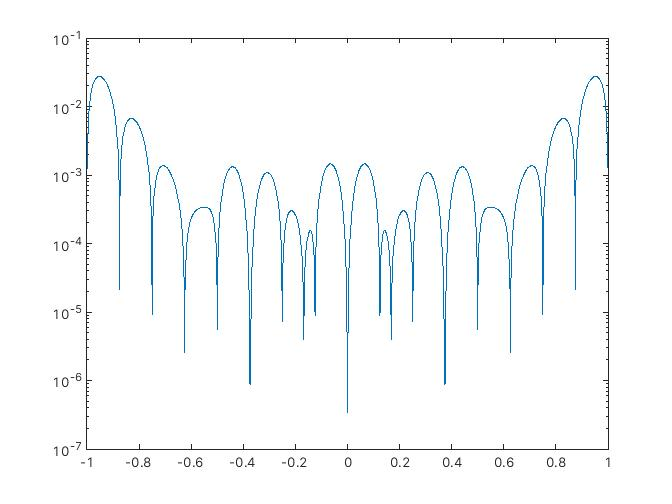
\includegraphics[width=15cm,height=8cm]{ex1d1.jpg}
   \caption{第一题(d) 逐点误差semilogy图}
\end{figure}

\begin{figure}[htbp]
   \centering
   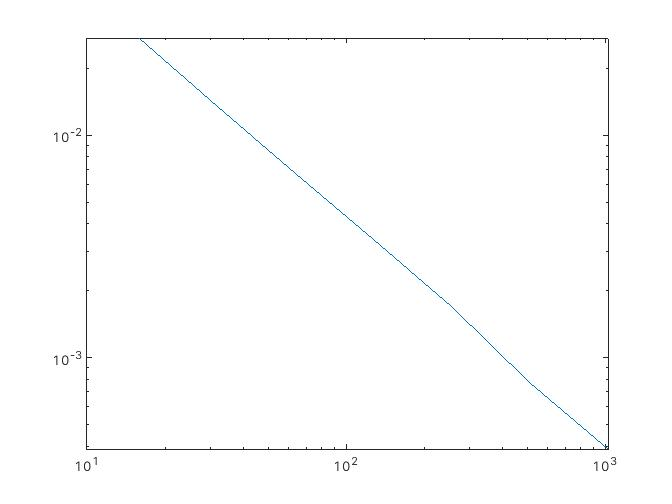
\includegraphics[width=15cm,height=8cm]{ex1d2.jpg}
   \caption{第一题(d) 最大误差loglog图}
\end{figure}

MATLAB程序如下:
\begin{lstlisting}[frame=single]
   n = 2^4; % 定义n
   x = [-1:2/n:1]; % 得到区间端点x_i
   % 得到h_i
   h=[];
   for i=1:n
       h=[h x(i+1)-x(i)];
   end 
   y=sin(4.*x.^2)+(sin(4.*x)).^2; % 得到y_i
   % 初始化lambda,mu,d
   lambda=ones(n,1);
   mu=ones(n,1);
   d=ones(n,1);
   % 对除端点的lambda,mu,d赋值
   for i=2:n
       lambda(i-1)=h(i)/(h(i)+h(i-1));
       mu(i-1)=1-lambda(i-1);
       d(i-1)=6/(h(i)+h(i-1))*((y(i+1)-y(i))/h(i) ... 
       -(y(i)-y(i-1))/h(i-1));
   end
   % 对端点的lambda,mu,d赋值
   d(n)=6/(h(1)+h(n))*((y(2)-y(1))/h(1) - (y(n+1)-y(n))/h(n));
   lambda(n)=h(1)/(h(1)+h(n));
   mu(n)=1-lambda(n);
   lambda2=lambda;
   lambda2(n)=[];
   mu2=mu;
   mu2(1)=[];
   % 得到求解M的系数矩阵A
   A=diag(mu2,-1)+2.*eye(n)+diag(lambda2,1);
   A(1,n)=mu(1);
   A(n,1)=lambda(n);
   M=A\d; 
   M=[M(n);M];%得到M
   x2=[-1:2/1999:1];% 分割2000个插值点
   S=zeros(1,size(x2,1));% 初始化S
   % 通过式(1)得到分段函数S
   for i=1:n
       S=S+ ...
       (((x(i+1)-x2).^3*M(i)+(x2-x(i)).^3*M(i+1))/6/h(i) ...
       +((x(i+1)-x2)*y(i)+(x2-x(i))*y(i+1))/h(i) ...
       -(h(i)/6)*((x(i+1)-x2)*M(i)+(x2-x(i))*M(i+1)) ...
       ).*(x2>x(i)&x2<=x(i+1));% 分段函数即所有函数值.*其区间最后求和
   end
   % 单独得到S(1)
   S(1)=((x(1+1)-x2(1)).^3*M(1)+(x2(1)-x(1)).^3*M(1+1))/6/h(1) ...
           +((x(1+1)-x2(1))*y(1)+(x2(1)-x(1))*y(1+1))/h(1) ...
           -(h(1)/6)*((x(1+1)-x2(1))*M(1)+(x2(1)-x(1))*M(1+1));
   y2=sin(4.*x2.^2)+(sin(4.*x2)).^2;% 真实值
   % 画图
   figure
   semilogy(x2,abs(y2-S))
   
   err_max=zeros(1,7);% 初始化误差
   n2=[];% n2储存n值
   for exp=4:10
       n = 2^exp;% 定义n
       x = [-1:2/n:1];% 得到区间端点x_i
       % 得到h_i
       h=[];
       for i=1:n
           h=[h x(i+1)-x(i)];
       end 
       y=sin(4.*x.^2)+(sin(4.*x)).^2; % 得到y_i
       % 初始化lambda,mu,d
       lambda=ones(n,1);
       mu=ones(n,1);
       d=ones(n,1);
       % 对除端点的lambda,mu,d赋值
       for i=2:n
           lambda(i-1)=h(i)/(h(i)+h(i-1));
           mu(i-1)=1-lambda(i-1);
           d(i-1)=6/(h(i)+h(i-1))*((y(i+1)-y(i))/h(i) ... 
           -(y(i)-y(i-1))/h(i-1));
       end
       % 对端点的lambda,mu,d赋值
       d(n)=6/(h(1)+h(n))*((y(2)-y(1))/h(1) - (y(n+1)-y(n))/h(n));
       lambda(n)=h(1)/(h(1)+h(n));
       mu(n)=1-lambda(n);
       lambda2=lambda;
       lambda2(n)=[];
       mu2=mu;
       mu2(1)=[];
       % 得到求解M的系数矩阵A
       A=diag(mu2,-1)+2.*eye(n)+diag(lambda2,1);
       A(1,n)=mu(1);
       A(n,1)=lambda(n);
       M=A\d; 
       M=[M(n);M];%得到M
       x2=[-1:2/1999:1];% 分割2000个插值点
       S=zeros(1,size(x2,1));% 初始化S
       % 通过式(1)得到分段函数S
       for i=1:n
           S=S+ ...
               (((x(i+1)-x2).^3*M(i)+(x2-x(i)).^3*M(i+1))/6/h(i) ...
               +((x(i+1)-x2)*y(i)+(x2-x(i))*y(i+1))/h(i) ...
               -(h(i)/6)*((x(i+1)-x2)*M(i)+(x2-x(i))*M(i+1)) ...
               ).*(x2>x(i)&x2<=x(i+1));
       end
       % 单独得到S(1)
       S(1)= ... 
         ((x(1+1)-x2(1)).^3*M(1)+(x2(1)-x(1)).^3*M(1+1))/6/h(1) ...
         +((x(1+1)-x2(1))*y(1)+(x2(1)-x(1))*y(1+1))/h(1) ...
         -(h(1)/6)*((x(1+1)-x2(1))*M(1)+(x2(1)-x(1))*M(1+1));
       y2=sin(4.*x2.^2)+(sin(4.*x2)).^2;% 真实值
       err_max(exp-3)=max(abs(y2-S));% 计算误差并保存
       n2=[n2 2^exp];
   end
   % 打印err_max结果
   err_max 
   % 画图
   figure
   loglog(n2,err_max,'-')
\end{lstlisting}

\newpage
\item[第二题]\textbf{本题深入讨论Newton插值公式的性质。}  

(a)(15分)对于一个光滑函数$ f(x) $ ,证明若$ {i_0, i_1,,\cdots , i_k} $ 是$ {0, 1, ..., k} $ 的任意一
个排列,则
$$f[x_0, x_1,,\cdots , x_k] = f[x_{i_0}, x_{i_1},,\cdots , x_{i_k}]$$ 

证:

先证一个结论:
$$ f[x_0, x_1,\cdots , x_k]=\sum_{i=0}^{k} \frac{f(x_i)}{(x_i-x_0)\cdots (x_{i}-x_{i-1})(x_{i}-x_{i+1})\cdots (x_i-x_k) }  $$
该结论可以通过归纳法证明。

$ f[x_0,x_1] $ 显然对上述结论成立。

假设k阶差商成立,则有:
$$ f[x_0, x_1,\cdots , x_k]=\sum_{i=0}^{k} \frac{f(x_i)}{(x_i-x_0)\cdots (x_{i}-x_{i-1})(x_{i}-x_{i+1})\cdots (x_i-x_k) } $$
$$ f[x_1, x_2,\cdots , x_{k+1}]=\sum_{i=1}^{k+1} \frac{f(x_i)}{(x_i-x_1)\cdots (x_{i}-x_{i-1})(x_{i}-x_{i+1})\cdots (x_i-x_{k+1}) } $$

对于k+1阶差商,有:
\begin{equation}
   \begin{split}
      & f[x_0, x_1,\cdots , x_{k+1}] = \frac{f[x_1, x_2,\cdots , x_{k+1}]-f[x_0, x_1, ..., x_k]}{x_{k+1}-x_0} \\
      & =\frac{\sum_{i=1}^{k+1} \frac{f(x_i)}{(x_i-x_1)\cdots (x_{i}-x_{i-1})(x_{i}-x_{i+1})\cdots (x_i-x_{k+1}) } - \sum_{i=0}^{k} \frac{f(x_i)}{(x_i-x_0)\cdots (x_{i}-x_{i-1})(x_{i}-x_{i+1})\cdots (x_i-x_k) }}{x_{k+1}-x_{0}} \\
      & =\frac{1}{x_{k+1}-x_0} (\frac{f(x_{k+1})}{(x_{k+1}-x_1)\cdots (x_{k+1}-x_k)} - \frac{f(x_{0})}{(x_0-x_1)\cdots (x_0-x_k)}\\
      & +\sum_{i=1}^{k}[\frac{f(x_i)}{(x_i-x_1)\cdots (x_i-x_{k+1}) } - \frac{f(x_i)}{(x_i-x_0)\cdots (x_i-x_k) }])\\
      & = \frac{1}{x_{k+1}-x_0} (\frac{f(x_{k+1})}{(x_{k+1}-x_1)\cdots (x_{k+1}-x_k)} - \frac{f(x_{0})}{(x_0-x_1)\cdots (x_0-x_k)}\\
      & +\sum_{i=1}^{k}[(\frac{1}{x_i-x_{k+1}} - \frac{1}{x_i-x_0})\frac{f(x_i)}{(x_i-x_1)\cdots (x_i-x_{k}) }])\\
      & =\sum_{i=0}^{k+1} \frac{f(x_i)}{(x_i-x_0)\cdots (x_{i}-x_{i-1})(x_{i}-x_{i+1})\cdots (x_i-x_{k+1}) }
      \notag
      \end{split}
   \end{equation}
由归纳假设,得证。

由上述结论:
\begin{equation}
   \begin{split}
      RHS& = \sum_{l=i_0, i_1,\cdots , i_k} \frac{f(x_l)}{(x_l-x_0)\cdots (x_{l}-x_{l-1})(x_{l}-x_{l+1})\cdots (x_l-x_k) } \\
         & = \sum_{i=0}^{k} \frac{f(x_i)}{(x_i-x_0)\cdots (x_{i}-x_{i-1})(x_{i}-x_{i+1})\cdots (x_i-x_k) } \\
         & = LHS
      \notag
      \end{split}
   \end{equation}

综上所述,本题得证。

(b)(10分)课堂上我们提到了Chebyshev点
$$ x_j = cos(jπ/n) j = 0, 1, ..., n $$
以及使用Chebyshev点可以有效地克服Runge现象。写一个Matlab程序,令$ n=2^2,2^3,...,2^7 $ 
,按照从右到左的顺序(即j从小到大的顺序)使用对应的n + 1个Chebyshev点对定义在[−1, 1]上的Runge函数
$$f(x) = \frac{1}{1+25x^2} $$
进行插值,并取2000个等距点上的误差的最大值,用semilogy图描述插值区间上最大误差值随n变化的情况(即横轴是n)。

解:

程序主要思路参照课本31、32页的伪代码。

程序结果如下:
\begin{figure}[htbp]
   \centering
   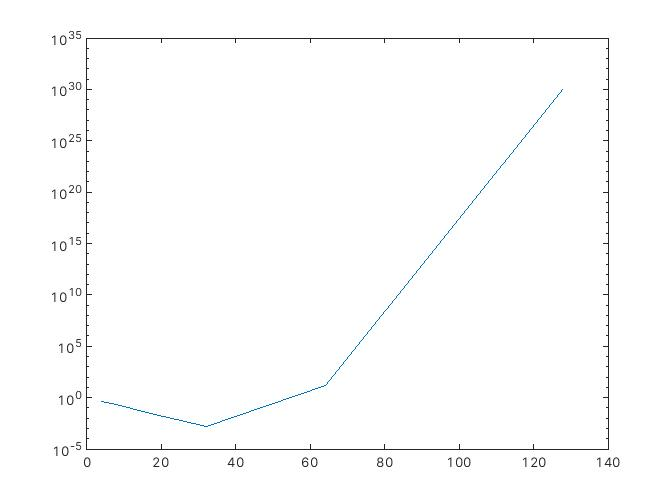
\includegraphics[width=15cm,height=8cm]{ex2b.jpg}
   \caption{第二题(b) 最大误差与n的semilogy图}
\end{figure}

MATLAB程序如下:
\begin{lstlisting}[frame=single]
u=[-1:2/1999:1];% 分割2000个插值点
y_real=1./(1.+25*u.^2);% 真实值
err_max=[];
n2=[];% n2储存不同n值
for exp=2:7
    n=2^exp;
    x=[];
    for j=0:n
        x=[x cos(j*pi/n)]; % Chebyshev点
    end
    y=1./(1+25*x.^2);
    % 形成差商表
    g=y;
    for k=1:n
        for j=n:-1:k
            g(j+1)=(g(j+1)-g(j))/(x(j+1)-x(j-k+1));
        end
    end
    % 得到newton插值函数
    t=1;
    newton=g(1);
    for k=1:n
        t=t.*(u-x(k));
        newton=newton+t*g(k+1);% 插值结果用newton储存
    end
    err_max=[err_max max(abs(newton-y_real))];
    n2=[n2 2^exp];
end
err_max;
% 画图
figure
semilogy(n2,err_max)
\end{lstlisting}

(c) (10分) 重复上一问,但使用随机数种子rng(22)和randperm函数来随机计算差商时插值点的使用顺序,取关于不同n的2000个等距点上的误差的最大值,用semilogy图描述插值区间上最大误差值随n变化的情况(即横轴是n)。

解:

程序与上一问基本相同,只需要在生成插值点后用rng和randperm函数打乱顺序即可。

程序结果如下:
\begin{figure}[htbp]
   \centering
   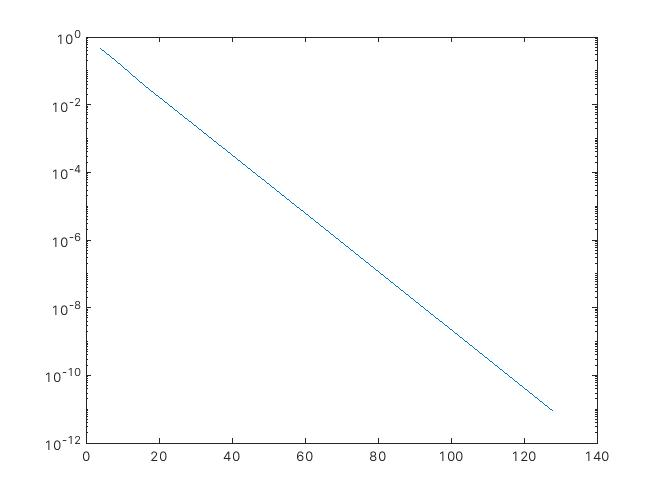
\includegraphics[width=15cm,height=8cm]{ex2c.jpg}
   \caption{第二题(b) 最大误差与n的semilogy图}
\end{figure}

MATLAB程序如下:
\begin{lstlisting}[frame=single]
   u=[-1:2/1999:1];% 分割2000个插值点
   y_real=1./(1.+25*u.^2);% 真实值
   err_max=[];
   n2=[];% n2储存n值
   for exp=2:7
       n=2^exp;
       x=[];
       for j=0:n
           x=[x cos(j*pi/n)];
       end
       % 改变插值点顺序
       rng(22);
       x=x(randperm(size(x,2)));
       y=1./(1+25*x.^2);
       % 形成差商表
       g=y;
       for k=1:n
           for j=n:-1:k
               g(j+1)=(g(j+1)-g(j))/(x(j+1)-x(j-k+1));
           end
       end
       t=1;
       newton=g(1);
       for k=1:n
           t=t.*(u-x(k));
           newton=newton+t*g(k+1);
       end
       err_max=[err_max max(abs(newton-y_real))];
       n2=[n2 2^exp];
   end
   err_max;
   % 画图
   figure
   semilogy(n2,err_max)
\end{lstlisting}

(d)(10分)试着解释上面两小问中你观察到的不同现象产生的原因。注:此问答不出来也无妨。

答:首先,由插值多项式的唯一性可知,在算法上改变插值点的顺序是不会改变插值结果的。
所以这种现象主要是因为近似计算过程中的舍入误差造成,即产生了龙格现象。
而舍入误差主要在每一项的差商计算和乘法计算中产生。
改变插值点顺序带来的乘法计算上的误差并不大,但对除法计算也就是差商的计算上会带来巨大影响。
在差商计算过程中,如果是按顺序取点,则在低阶差商上分母的值非常的小,
有可能其浮点数精度误差数量级相当,这就导致误差对式子的值产生了不可忽略的影响。
而打乱顺序后,分母是插值点随机两个数的差,在某种取值条件下就可能会避免出现两个数十分接近的情况,
舍入误差就会变小。
而截断误差会随着n的增大而减小,所以打乱插值点顺序可以让误差随n的增大而减小;
而按原顺序插值在低阶拟合下舍入误差小于截断误差,所以误差会先随n增大而减小,
随着n越来越大,上述提到的舍入误差越来越大,最后舍入误差的影响大于截断误差,误差就会反弹,
所以就出现了图5、图6的现象。





\newpage
\item[第三题]\textbf{本题用于讨论周期函数的Lagrange插值方法。对于周期函数而言,多项式不再是最有效的基函数,而等距插值点也不再会出现Runge现象。逼近周期函数的基函数通常选用三角函数或者复指数。同时注意对于周期函数而言,插值点数量和子区间个数相等。}  

(a) (10分)在[0, 1]上关于周期函数的基于等间距插值点$ x_j =\frac{j}{n} , j = 0, 1, ...,n − 1 $ 的Lagrange插值基函数为

\begin{equation}
    \ell_{k}(x)=\left\{\begin{array}{ll}
    \frac{(-1)^{k}}{n} \sin (n \pi x) \csc \left(\pi\left(x-x_{k}\right)\right) & \text { 若 } n \text { 为奇数 } \\
    \frac{(-1)^{k}}{n} \sin (n \pi x) \cot \left(\pi\left(x-x_{k}\right)\right) & \text { 若 } n \text { 为偶数 }
    \end{array}\right.\notag
    \end{equation}

证明对于n分别为奇数和偶数的情况下
\begin{equation}
    \ell_{k}\left(x_{j}\right)=\left\{\begin{array}{ll}
    1 & k=j \\
    0 & k \neq j
    \end{array}\right.\notag
\end{equation}

证:

n为奇数时:

当$ k\neq j $ 有
$$ sin(n\pi x_j)=sin(n\pi \frac{j}{n} )=0,csc(\pi (x_j-x_k))=csc(\pi \frac{j-k}{n} )\neq \infty $$
故此时$ l_k(x_j)=0 $ .


当$ k=j $ 有
$$ sin(n\pi x_j)=sin(n\pi \frac{j}{n} )=0,csc(\pi (x_j-x_k))=csc(\pi \frac{j-k}{n} )= \infty $$
故此时
$$ l_k(x_j)= \frac{(-1)^k}{n} \lim_{x \to x_k} \frac{sin(n\pi x)}{sin(\pi (x-x_k))}=\frac{(-1)^k}{n}\lim_{x \to x_k} \frac{ncos(n\pi x)}{cos(\pi(x-x_k))}=1 $$

n为偶数时:

同理

当$ k\neq j $ 有
$$ sin(n\pi x_j)=sin(n\pi \frac{j}{n} )=0,cot(\pi (x_j-x_k))=cot(\pi \frac{j-k}{n} )\neq \infty $$
故此时$ l_k(x_j)=0 $ .

当$ k=j $ 有
$$ sin(n\pi x_j)=sin(n\pi \frac{j}{n} )=0,cot(\pi (x_j-x_k))=cot(\pi \frac{j-k}{n} )= \infty $$
故此时
$$ l_k(x_j)= \frac{(-1)^k}{n} \lim_{x \to x_k} \frac{sin(n\pi x)}{tan(\pi (x-x_k))}=\frac{(-1)^k}{n}\lim_{x \to x_k} \frac{ncos(n\pi x)}{\frac{1}{cos^2(\pi(x-x_k))} }=1 $$

综上所述,有
\begin{equation}
    \ell_{k}\left(x_{j}\right)=\left\{\begin{array}{ll}
    1 & k=j \\
    0 & k \neq j
    \end{array}\right.\notag
\end{equation}


(b)(10分)用上述对应于n为偶数的Lagrange基函数构造Lagrange插值多项式,并用$ n = 2^6 $ 个点对周期函数
$ f(x) = sin(2πx)e^{cos(2πx)} $ 在[0, 1]上进行插值。
取1000个等距点上的误差,用semilogy图描述插值区间上误差值随x变化的情况(即横轴是x)。

解:

程序思路:

通过上述插值点得到$ l_k(x) $ 函数的参数,然后作组合
$$ L_n(x)=\sum_{i=0}^{n}l_i(x)f(x_i) $$
即可得到插值函数。

具体伪代码可以参见书p24页伪代码,只需将其中的插值基函数改为本题中的基函数即可。

\newpage
得到的结果图如下
\begin{figure}[h]
    \centering
    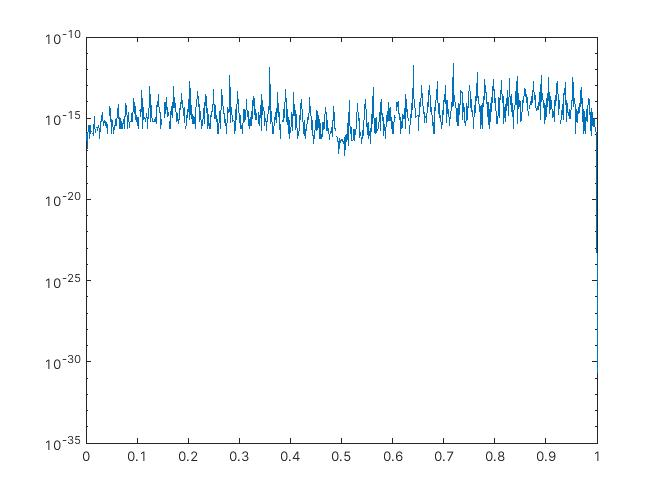
\includegraphics[width=15cm,height=7cm]{ex3b.jpg}
    \caption{第三题(b) 误差随x变化的semilogy图}
 \end{figure}


MATLAB程序如下:
\begin{lstlisting}[frame=single]
    n=2^6;
    u=[0:1/999:1];% 取1000个等距点
    y_real=sin(2*pi*u).*exp(cos(2*pi*u));% 真实值
    x=[0:1/n:(n-1)/n];
    y=sin(2*pi*x).*exp(cos(2*pi*x));
    y_pred=zeros(size(u));
    for k=1:n
        y_pred=y_pred+ ...
            y(k)*((-1)^(k-1)*sin(n*pi*u) ...
            .*cot(pi*(u-x(k))))/n ...
            .*(~ismembertol(u,x,1e-6)) ...
            +y(k).*(ismembertol(u,x,1e-6));
    end
    err = abs(y_pred-y_real);
    figure
    semilogy(u,err)
\end{lstlisting}

\newpage
\item[第二题]\textbf{(10分) 写程序完成课本59页第7题,并计算出你的拟合函数对比所给数据点的误差的2-范数}

MATLAB程序如下:
\begin{lstlisting}[frame=single]
    % 初始化x,y
    y=[0.6087;0.6849;0.7368;0.8111];
    x=[2.1;2.5;2.8;3.2];
    % 对x,y每个元素取倒数
    y_inv=1./y;
    x_inv=1./x;
    A=[ones(size(x)) x_inv];% 得到A矩阵
    Y=y_inv;% 得到Y矩阵
    b_a=(A'*A)\(A'*Y);% 通过最小二乘法得到a,b
    % 输出a,b的值
    a=b_a(2)
    b=b_a(1)
    y_pred=x./(b_a(1).*x+b_a(2));% 得到预测的y值
    l2=norm(y-y_pred)% 计算2-范式并打印
\end{lstlisting}

程序结果如下:
\begin{lstlisting}[frame=single]
    >> ex4

    a =
    
        2.4867
    
    
    b =
    
        0.4623
    
    
    l2 =
    
        0.0060
\end{lstlisting}







\end{enumerate}




\end{document}
